\section{Construcción canónica}

Comenzamos planteando algunas definiciones.

\subsection{Discretización puntual, polinomios discretos y espacios asociados}
\label{discretizacion puntual, polinomios discretos y espacios asociados}

\begin{marginfigure}
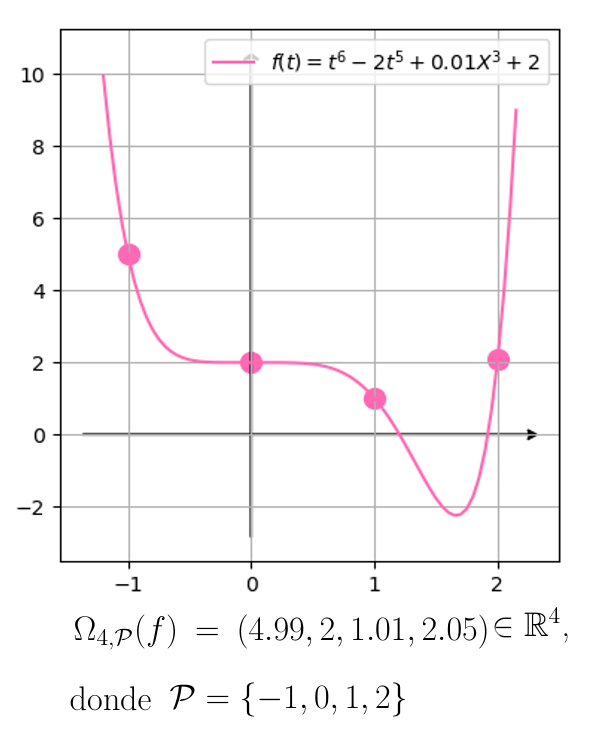
\includegraphics[scale=0.9]{1En_1} 
		\caption{Ejemplo concreto con $n=4$.}
\end{marginfigure}


\begin{defi}
\label{def: operador de discretizacion puntual}
(\textbf{Operador de discretización} $\Omega_{n,\cali{P}}$)
Sea $\cali{P}$ una malla uniforme 
de $n$ puntos
\[
\cali{P}:=\{ t_{j}:=t_{0}+hj : \hspace{0.1cm} 0 \leq j \leq n-1 \},
\]
donde $h \in \IR^{+}$ es una constante fija
(que llamamos el \textbf{paso} de la malla).
Nuestra primera forma de discretizar
a una función $f$ cuyo dominio contenga a los puntos
de la malla $\cali{P}$
consistirá en evaluarla en cada uno de los
puntos de la malla:

\begin{center}
$\Omega_{n,\cali{P}}(f) := (f(t_{j}))_{j=0}^{n-1}.$
\end{center}
\end{defi}


%\begin{figure}[H]
%\centering\captionsetup{format = hang}
%	\begin{measuredfigure}
%		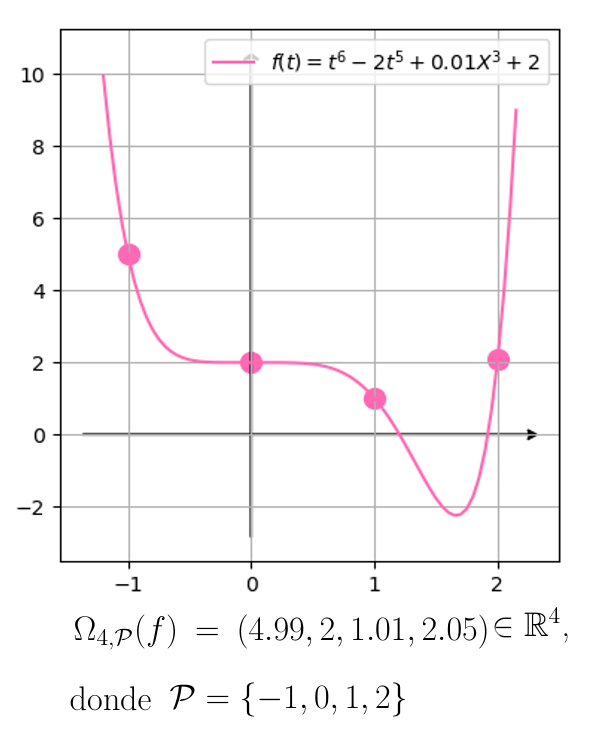
\includegraphics[scale=1.3]{1En_1} 
%		\caption{Ejemplo concreto con $n=4$.}
% 	\end{measuredfigure}
% \end{figure}

\noindent $\Omega_{n,\cali{P}}$
puede pensarse como una aplicación con dominio
$\cali{C}[t_{0}, t_{n-1}]$,
el espacio de funciones 
continuas en $[t_{0}, t_{n-1}]$,
y con codominio $\IR^{n}$, pero conviene 
identificar al resultado 
de la acción de $\Omega_{n,\cali{P}}$ sobre una
función $f$ con la restricción $f_{| \cali{P}}$
de 
$f$ al conjunto discreto $\cali{P}$,
es decir, con la función

\begin{center}
\aplica{f_{|\cali{P}}}
{\cali{P}}
{\IR }
{t_{j}}{f(t_{j}).}
\end{center}



\begin{defi} \label{def: polinomio discreto}
En el caso en el que $f$ sea elemento de $\IR[x]$, 
nos referiremos
al vector $\Omega_{n,\cali{P}}(f) \in \IR^{n}$
como un \textbf{polinomio discreto
de dimensión $n$ con dominio uniforme $\cali{P}$.} 
\end{defi} 

\sidenote{
En lo que sigue, siempre que se hable de un polinomio
discreto
se supondrá que la malla $\cali{P}$
a partir de la que se obtuvo es uniforme.}


Mostraremos en la subsección
\ref{definicion del concepto de grado para seniales finitas}
que, de hecho, \textbf{todo}
$x \in \IR^{n}$ es un polinomio discreto,
y daremos una definición del grado de este.
Ya podríamos dar algunos resultados en esta dirección,
pero preferimos esperar hasta tener las herramientas
para justificar detalles como la buena definición
de nuestra propuesta de grado.


Por la forma en que se definen la suma y la multiplicación
por escalares en los espacios vectoriales $\IR[x]$
y $\IR^{n}$, la siguiente observación es clara.

\begin{obs} \label{obs:linealidad de omega restringida a R[x]}
Sean $n \in \IN$ y $\cali{P}=\{t_{j}:
\hspace{0.2cm}0 \leq j \leq n-1 \}$ una malla uniforme
de $n$ puntos.
La función $\Omega_{n , \cali{P}}$ 
definida en 
\ref{def: operador de discretizacion puntual}
es una transformación lineal de 
$\cali{C}[t_{0}, t_{n-1}]$ a $\IR^{n}$.
\end{obs}
 


\begin{notacion} \label{notacion: Pn, fk, Wi, vk}
Sea $n \in \IN$ y $k$ un entero no negativo.
\footnote{Como se verá más adelante, 
nos interesarán sólo los enteros $k$
con $0 \leq k \leq n-1$.}.Denotaremos 
por $\IR_{k}[x]$ al subespacio de $\IR[x]$
que consta de los polinomios de grado a lo más $k$.
\noindent
Escribiremos como $f_{k}$ 
a las potencias básicas,
es decir, a los polinomios
\begin{equation}
\label{fk}
f_{k}(t):=t^{k}.
\end{equation}
Denotaremos por $\cali{P}_{n}$ a la siguiente
malla uniforme:
\begin{equation}
\label{malla Pn}
\cali{P}_{n}=\{ 0, 1, \ldots , n-1 \}.
\end{equation}
A la discretización puntual del
polinomio $f_{k}$ en la malla 
$\cali{P}_{n}$
la denotaremos por $v_{k}$;
\begin{equation}
\label{vectores vk}
v_{k}:= \Omega_{n, \cali{P}_{n}}(f_{k})
=(f_{k}(j))_{j=0}^{n-1}=(j^{k})_{j=0}^{n-1},
\end{equation}
y al subespacio de $\IR^{n}$ generado por los
primeros $i+1$ vectores $v_{k}$
(con $0 \leq i \leq n-1$ entero)
por por $W_{n,i}$;
\begin{equation}
\label{espacios Wi}
W_{n,i} := span\{ v_{k} : 0 \leq k \leq i \} \subseteq \IR^{n}.
\end{equation}
\end{notacion}


En la ecuación \eqref{espacios Wi} con la que se
define al espacio $W_{n,i}$,
siempre conviene pensar al primer subíndice $n$
como el \textbf{índice de dimensión}, pues corresponde
a la dimensión del espacio ambiente $\IR^{n}$,
y al subíndice $i$ como \textbf{índice de grado};
más adelante (c.f. tercer punto del teorema 
\ref{cor: propiedades importantes de espacios Wi}) 
se verá por qué este es un buen nombre.



\begin{obs} \label{obs:independencia lineal polinomios}
Sea $n \in \IN$. Si $i \in \overline{\IN}$, entonces
los $i+1$ polinomios
$f_{k}$ con $0 \leq k \leq i$ entero
constituyen una base para el espacio $\IR_{i}[x]$.
\end{obs}


\noindent
Como veremos a continuación, 
nuestras motivaciones geométricas
iniciales (el saber si la gráfica de una señal
de dimensión $n$ es afín o cuadrática) 
pueden reformularse en términos
de pertenencia a los espacios $W_{n,i}$.


\begin{prop} \label{obs: s en Wi sii es la discretizacion en malla Pn de un pol de grado a lo más i}
Sea $n \in \IN$.
Una señal $x=(x_{k})_{k=0}^{n-1}$ de dimensión $n$
es elemento del espacio $W_{n,i}$ 
definido en \eqref{espacios Wi}
si y sólo si 
$x$ es la discretización en $\cali{P}_{n}$
de un polinomio de grado a lo más $i$.
\end{prop}
\noindent
\textbf{Demostración.}
En efecto, según la definición del espacio
$W_{n,i}$ y la linealidad del operador
de discretización 
$\Omega$ establecida en 
la observación
\ref{obs:linealidad de omega restringida a R[x]}, 
tenemos que $x \in \IR^{n}$ es elemento de 
$W_{n,i}$ si y sólo si existen números reales
$a_{k}$ con $0 \leq k \leq i$ tales que
\begin{align*}
x=  \suma{k=0}{i}{a_{k}v_{k}} 
=  \suma{k=0}{i}{a_{k}\Omega_{n, \cali{P}_{n}}(f_{k})}
=  \Omega_{n, \cali{P}_{n}} \left( 
\suma{k=0}{i}{a_{k}f_{k}} \right)
=  \Omega_{n, \cali{P}_{n}} (g),
\end{align*}
con $g := \suma{k=0}{i}{a_{k}f_{k}} \in \IR_{i}[x]$
(c.f. observación 
\ref{obs:independencia lineal polinomios}).
\null\nobreak\hfill\ensuremath{\square} %final dem


\begin{cor} \label{cor: condiciones necesarias y suficientes para que x sea afín en términos de pertenencia a espacios Wi}
Sean $n \in \IN$ y $x \in \IR^{n}$ una señal de dimensión
$n$ cualquiera.
\begin{itemize}
\item La señal $x$ es constate si y sólo si $x \in W_{n,0}$,

\item es afín si y sólo si $x \in W_{n,1}$, y 

\item es cuadrática si y sólo si $x \in W_{n,2}$
y $x \not\in W_{n,1}$. \TODO{el último punto es claro? Tal vez lo sea
si este corolario va después.}
\end{itemize}
\end{cor}
\noindent
La importancia del corolario
\ref{cor: condiciones necesarias y suficientes para que x sea afín en términos de pertenencia a espacios Wi}
es que en él se explica cómo
\textbf{cuestiones de morfología de la señal $x$
se reducen a cuestiones de pertenencia a los espacios $W_{n,i}$}.
Parece pues que los espacios $W_{n,i}$ son un buen lugar
en el que buscar una base ortonormal con las propiedades
descritas en la lista 
de objetivos \ref{lista de objetivos}.

\noindent Demostremos ahora que,
en la proposición
\ref{obs: s en Wi sii es la discretizacion en malla Pn de un pol de grado a lo más i},
poco importa
la malla sobre la que se discretice, siempre y
cuando esta sea uniforme.


\begin{prop} \label{Obs1}
Si $\cali{P}$ es una malla
uniforme cualquiera de $n$ puntos, digamos
\[
\cali{P}= \{ t_{j}:= t_{0}+h :\hspace{0.1cm} 0 \leq l \leq n-1 \},
\]
con $h$ una constante positiva, 
y $f$ es un polinomio de grado $i$
(con $0 \leq i \leq n-1$),
entonces el vector $\Omega_{n, \cali{P}}(f)$ de $\IR^{n}$ 
es elemento del espacio $W_{n,i}$ definido en 
\eqref{espacios Wi}.
\end{prop}
\noindent
\textbf{Demostración.}
Según la observación \ref{obs:independencia lineal polinomios},
existen 
(únicos) números reales $c_{k}$, con $0 \leq k \leq i$
tales que 
$f= \suma{k=0}{i}{c_{k}f_{k}}$.
Sean los intervalos
\[
I_{n}=[0,n-1], \hspace{0.2cm} I=[x_{0}, x_{n-1}].
\]
Sea $\phi:I_{n} \longrightarrow I$ la función cuya gráfica
es el segmento de recta con puntos extremos 
\[
(0, t_{0}) \hspace{0.2cm} \text{y} \hspace{0.2cm}
(n-1, t_{n-1});
\]
la ecuación de tal $\phi$ es
\[
\phi(t)=ht+t_{0};
\] observe que $\phi$
es una recta con pendiente $h$ positiva.
Como tanto
$\cali{P}_{n}$ como $\cali{P}$
son mallas uniformes, 
\[
\forall \hspace{0.2cm} 0 \leq j \leq n-1: \hspace{0.2cm} \phi(j)=t_{j}.
\] 
(para convencerse de que esto ocurre
basta aplicar un argumento de semejanza de triángulos).
\noindent Así, la $(j+1)$-ésima entrada del
vector $\Omega_{n, \cali{P}}(f)=(f(t_{j}))_{j=0}^{n-1}$ es
\[
f(t_{j})= f (\phi (j))=
f(hj+t_{0})=
\suma{k=0}{i}{c_{k}f_{k}(hj+t_{0})}
= \suma{k=0}{i}{c_{k}(hj+t_{0})^{k}}.
\]
Reconocemos al lado derecho de la igualdad como un polinomio
de grado a lo más $i$, a saber,
\[
h(x):= \suma{k=0}{i}{c_{k}(hx+t_{0})^{k}}
\]
evaluado en el $(j+1)$-ésimo elemento 
de la malla uniforme $\cali{P}_{n}$
(o sea, en $j$). Según la observación
\ref{obs: s en Wi sii es la discretizacion en malla Pn de un pol de grado a lo más i}
de esto podemos concluir la pertenencia de 
$\Omega_{n, \cali{P}}(f)$ a $W_{n,i}$. \\

\begin{figure}[H]
	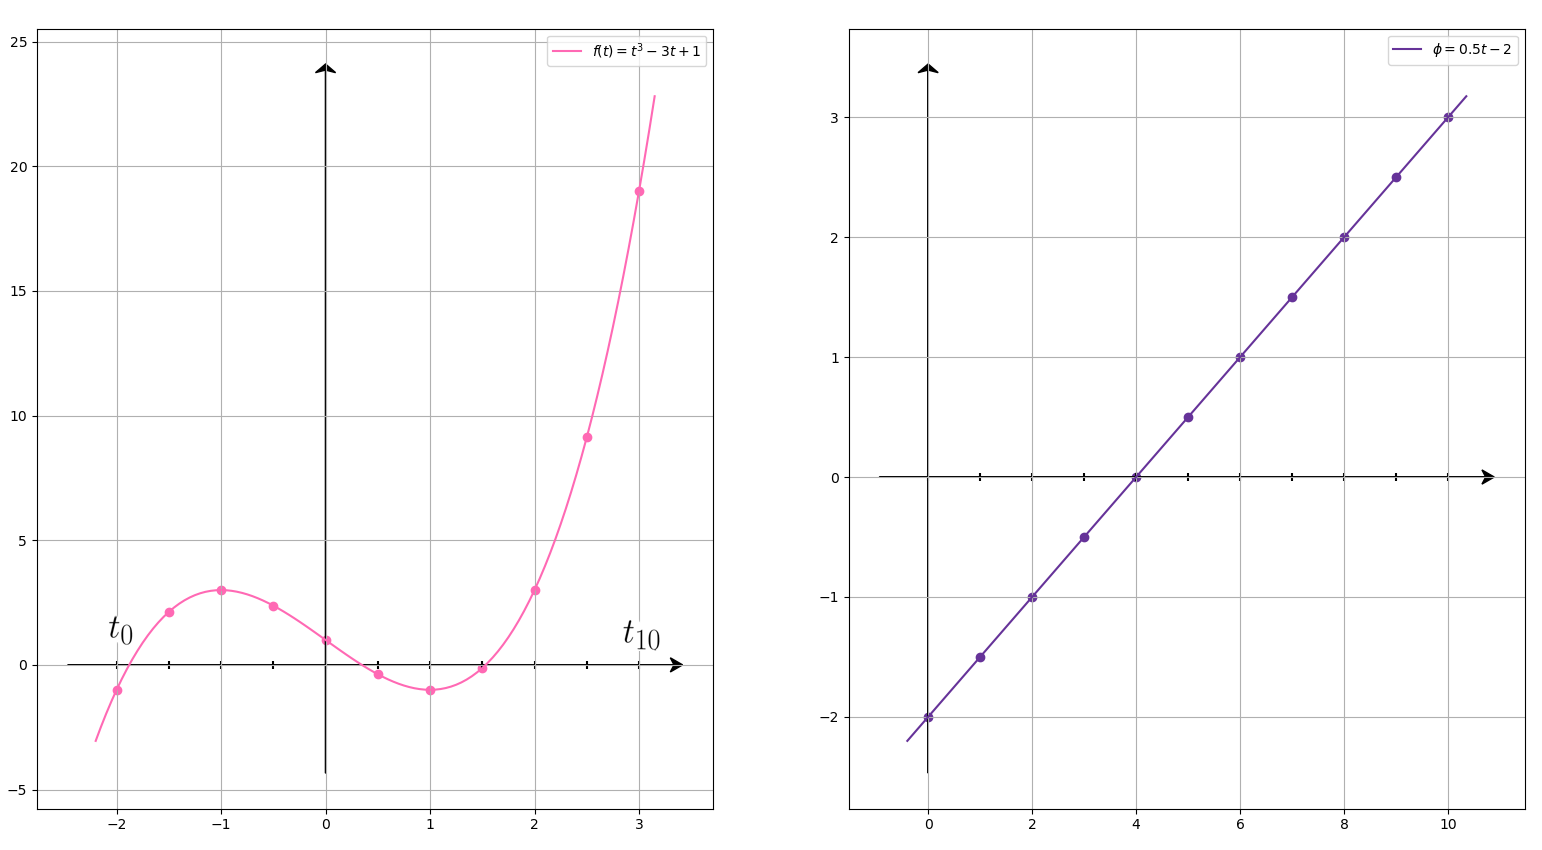
\includegraphics[scale=0.3]{mall} 
	\sidecaption{
	Ejemplo haciendo $n=11$, $\cali{P}$ la malla
	uniforme de $11$ puntos con punto inicial $-2$
	y paso $h=0.5$.	    
	A la izquierda se dibuja la gráfica de 
	$f(t)=t^{3}-3t+1$
	y su discretización puntual en $\cali{P}$.
	A la derecha, la gráfica de $\phi(t)=0.5t-2$. A  
    una tal función lineal $\phi$ le llamaremos, en este contexto,
    \textbf{función de cambio de malla}.}
 \end{figure}
\QEDB
\vspace{0.2cm}

Concluimos así que
el subespacio de $\IR^{n}$
\begin{equation*}
\label{def de espacios Wk}
W_{n,i}= span\{ v_{k} : 0 \leq k \leq i \},
\end{equation*}
con $0 \leq i \leq n-1$ entero,
\textbf{es} el espacio de
los polinomios discretos
de dimensión $n$ con dominio uniforme 
\sidenote{
Una contención se 
prueba en la proposición 
\ref{obs: s en Wi sii es la discretizacion en malla Pn de un pol de grado a lo más i}
y la otra en la proposición \ref{Obs1}.
}
y
de grado a lo más $i$.



Como mostramos en el siguiente teorema, los vectores
$v_{k}$, con $0 \leq k \leq i$, más que un conjunto generador
del espacio $W_{n,i}$, conforman una base de este.


\begin{prop} \label{Teorema1}
Sea $n \in \IN$.
Si $0 \leq i \leq n-1$ es un entero y
\[
\{ p_{k}=p_{k}(t): \hspace{0.2cm} 0 \leq k \leq i \}
\]
es una colección de polinomios linealmente independientes, con
\[
\partial (p_{k})=k, \hspace{0.4cm} 0 \leq k \leq i
\]
y 
\[
\cali{P}= \{ t_{j}= t_{0}+hj :\hspace{0.1cm} 0 \leq j \leq n-1 \}
\]
es una malla uniforme cualquiera
de $n$ puntos, entonces los $i+1$ vectores
de $\IR^{n}$
\begin{equation}
\label{eq1: 30Oct}
w_{k} := \Omega_{n, \cali{P}}(p_{k}), \hspace{0.4cm} 0 \leq k \leq i
\end{equation}
son linealmente independientes.
\end{prop}
\noindent
\textbf{Demostración.}
Mostremos primero que $\{ w_{k}: \hspace{0.1cm} 0 \leq k \leq i \}$
es un subconjunto linealmente independiente de $\IR^{n}$.
Sean $b_{k}$ con $0 \leq k \leq i$ escalares
para los que se tenga la siguiente igualdad en $\IR^{n}$:

\begin{equation} \label{eq1: 3Agosto}
\suma{k=0}{i}{b_{k}w_{k}}=0.
\end{equation}

\noindent 
Según la linealidad establecida en la observación
\ref{obs:linealidad de omega restringida a R[x]}
y la definición \ref{eq1: 30Oct} de los vectores $w_{k}$,
si $p=p(t)$ es el polinomio
definido como
\begin{equation}
\label{eq2: 30Oct}
p:=\suma{k=0}{i}{b_{k}p_{k}},
\end{equation}
la ecuación \eqref{eq1: 3Agosto} puede reescribirse como

\begin{equation} \label{eq2: 3Agosto}
\Omega_{n , \cali{P}} (p) = 0.
\end{equation}

Ahora bien, 
la ecuación \eqref{eq2: 3Agosto}
expone a los $n$ puntos
de la malla $\cali{P}$ como raíces de $p$;  puesto que
el grado de $p$ es menor a $n$
(pues $p$ se ha definido en \eqref{eq2: 30Oct} como
combinación lineal de polinomios de grado menor
a $n$), 
concluimos, según la proposición \ref{prop: cita TFA},
que $p$ es el polinomio cero, 
y de esto, por la
independencia lineal de los polinomios $p_{i}$
en el espacio $\IR[x]$, la
igualdad a cero de los escalares $b_{k}$. 
\QEDB
\vspace{0.2cm}

\begin{prop}
Sea $n \in \IN$. Para todo entero $0 \leq i \leq n-1$, 
$\{v_{k}: \hspace{0.1cm} 0\leq k \leq i \}$ es una base
del espacio $W_{n,i}$
definido en \eqref{espacios Wi}.
\end{prop}
\noindent
\textbf{Demostración.}
Puesto que los polinomios $f_{k}$, con $0 \leq k \leq i$
satisfacen las hipótesis de la proposición \ref{Teorema1},
según este resultado
tenemos que los vectores $v_{k}= \Omega_{n, \cali{P}_{n}}(f_{k})$ 
con $0 \leq k \leq i$
son linealmente independientes; como estos, 
por definición,
generan al espacio $W_{n,i}$, concluimos que 
estos conforman una base de $W_{n,i}$.
\QEDB
\vspace{0.2cm}

Las propiedades más importantes de los
espacios $W_{n,i}$ (y que se desprenden
de los argumentos anteriores) se 
resumen en el siguiente teorema. 
Sólo del notar que las dimensiones de 
$\IR^{n}$ y su subespacio $W_{n, n-1}$
coinciden se deduce el cuarto punto.

\TODO{Por aquí di que a $W_{n,0}$ le llamarás
el espacio de $n-$dimensionales ctes etc... y en una
sidenote que, a pesar de que en $W_{n,2}$ puede haber señales
que no son cuadráticas (sino ctes y afines) usas ese nombre
para dar a entener euq en $W_{n,2}$ hay, a lo más, de grado 2.
Cuidado; aún no hablas del grado de una señal. Entonces, mejor
pon esto justo después.}

\begin{teo}
\label{cor: propiedades importantes de espacios Wi}
Sea $n \in \IN$. Sean, para cada $0 \leq i \leq n-1$,
los espacios $W_{n,i}$ como
se definieron en \eqref{espacios Wi}.
\begin{itemize}
\item Para toda $i$, $W_{n,i}$ es un subespacio
de $\IR^{n}$ de dimensión $i+1$. De hecho, 
$\{v_{k}: \hspace{0.1cm} 0\leq k \leq i \}$, con
$v_{k}$ definido como en \eqref{vectores vk},
es base de $W_{n,i}$.

\item La familia $(W_{n,i})_{i=0}^{n-1}$ de subespacios
	de $\IR^{n}$ está estríctamente anidada, es decir
	\begin{equation}
	\label{espacios Wi estan anidados}
	\forall \hspace{0.1cm}
	0 \leq i \leq n-2: \hspace{0.2cm}
	W_{n,i} \subsetneq W_{n,i+1}.
	\end{equation}

\item El espacio $W_{n,i}$ consta \textbf{exactamente}
de los polinomios discretos de dimensión $n$ con dominio uniforme
de grado a lo más $i$.

\item $\IR^{n}= W_{n,n-1}$.
\end{itemize}
\end{teo}

\begin{figure}[H]
\centering\captionsetup{format = hang}
	\begin{measuredfigure}
		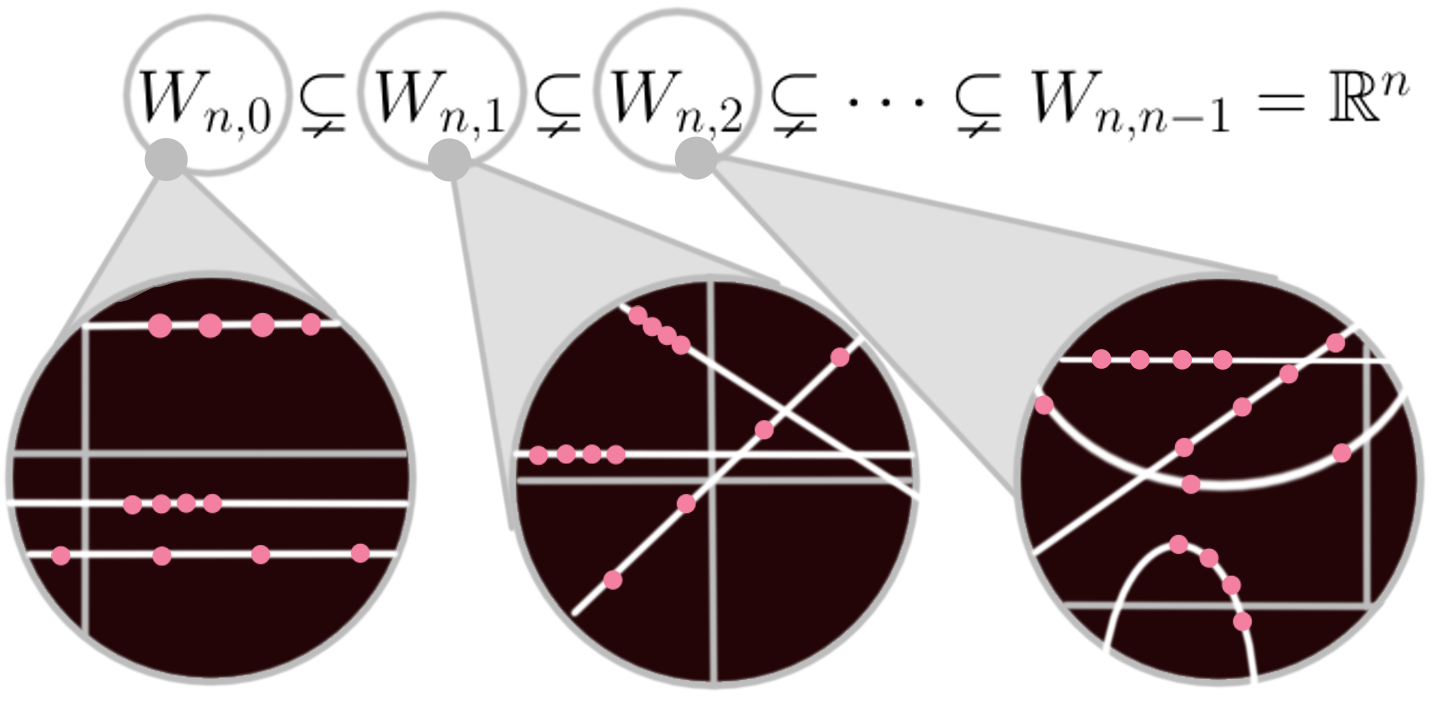
\includegraphics[scale=1]{nuevas_lupas} 
		\caption{
	En la figura	
	se dibujan las gráficas de algunos de los elementos
	de los tres primeros espacios de polinomios discretos
	$W_{n,0}$, $W_{n,1}$ y $W_{n,2}$
	(en la figura se ha fijado $n=4$).
    Observe que estas son
	las formas de recta y parábola de
	nuestro interés. 
	Queremos hacer énfasis en que, tomando
	\textbf{cualquier} malla uniforme y \textbf{cualquier} 
	polinomio $f$
	de grado $0 \leq i \leq n-1$, estamos seguros de que
	la discretización $\Omega_{n, \cali{P}}(f)$ es elemento
	del subespacio $W_{n,i}$ de $\IR^{n}$; reciprocamente, el 
	saber que un $x \in \IR^{n}$ sea elemento 
	de algún espacio $W_{n,i}$ (hecho
	que, en vistas de que la familia $(W_{n,i})_{i=0}^{n-1}$
	``cubre de manera ascendente a todo el espacio $\IR^{n}$''
	(c.f. puntos dos y cuatro del teorema 
	\ref{cor: propiedades importantes de espacios Wi}), seguro 
	ocurrirá), nos permite hacer inferencias sobre la forma 
	de la gráfica de $x$.}
 	\end{measuredfigure}
 \end{figure}





\subsection{Una definición del concepto de grado para señales finitas}
\label{definicion del concepto de grado para seniales finitas}

Revise nuevamente el último punto del teorema
\ref{cor: propiedades importantes de espacios Wi}; según este,
como se anticipó en la subsección 
\ref{discretizacion puntual, polinomios discretos y espacios asociados},
toda señal finita $x \in \IR^{n}$
es elemento de $W_{n,n-1}$,
es decir, es un polinomio discreto
de dimensión $n$ y grado menor a $n$.

Podemos dar una demostración
alternativa,
directa y sencilla de este hecho.

\begin{prop}
\label{prop: el operador de discretizacion puntual es un isomorfismo (...)}
Sean $n \in \IN$, $\cali{P}$ una malla uniforme de $n$
puntos. 
La restricción del operador $\Omega_{n, \cali{P}}$
al espacio $\IR_{n-1}[x]$ de polinomios de grado a lo más
$n-1$, es decir, la función 
\begin{equation}
\label{eq0: 28Nov}
\Omega_{n, \cali{P}}:
\IR_{n-1}[x] \longrightarrow \IR^{n}
\end{equation}
es un isomorfismo de $\IR-$espacios vectoriales.
En particular, para todo vector $x \in \IR^{n}$
existe un único polinomio $f$ de grado menor a n
tal que $x = \Omega_{n, \cali{P}}(f)$.
\end{prop}
\noindent
\textbf{Demostración.}
Puesto que tanto $\IR_{n-1}[x]$
como $\IR^{n}$ son $\IR$-espacios vectoriales
de dimensión $n$, para ver que la función 
\eqref{eq0: 28Nov} (que, según la observación 
\ref{obs:linealidad de omega restringida a R[x]}, es lineal)
es un isomorfismo, basta
demostrar que es inyectiva 
(c.f. teorema 2.5 \TODO{Friedberg}).
Esto último es una consecuencia directa del 
teorema fundamental del álgebra,
pues, 
$f \in \IR_{n-1}(x)$
es elemento del kernel
de \eqref{eq0: 28Nov} si y sólo si 
$\Omega_{n, \cali{P}}(f)=0$, o, equivalentemente,
si y sólo si 
cada uno de los $n$ puntos que componen la
malla $\cali{P}$ es una raíz de $f$. Puesto que
$f$ es un polinomio de grado a lo más $n-1$
(y, por lo tanto, de no ser el polinomio cero tiene
a lo más $n-1$ raíces reales),
esto último ocurre si y sólo si $f$ es el polinomio cero.
Con esto comprobamos que el kernel de la aplicación
\label{eq1: 25Nov} es trivial, luego, la inyectividad
de esta.
\QEDB
\vspace{0.2cm}

La proposición
\ref{prop: el operador de discretizacion puntual es un isomorfismo (...)}
parece sugerir 
una forma en la que podríamos 
definir el grado de 
un vector $x \in \IR^{n}$ (``dado $x \in \IR^{n}$, definimos
el grado de este como el grado del único polinomio $f \in \IR_{n-1}[x]$
tal que $\Omega_{n, \cali{P}}(f)=x$''); no hay
que apresurarse, pues en la formulación de
la proposición
\ref{prop: el operador de discretizacion puntual es un isomorfismo (...)}
se tuvo que fijar de antemano una malla uniforme.
\textit{A priori}, no podríamos descartar 
la existencia de mallas uniformes
$\cali{P}, \tilde{\cali{P}}$ 
de $n$ puntos
y de polinomios
$f, \tilde{f}$ de grados menores a $n$ (pero no 
iguales entre sí), tales que
$\Omega_{n, \cali{P}}(f) = x = \Omega_{n, \tilde{\cali{P}}}(\tilde{f})$.
Comprobamos que esto no ocurre
en el siguiente resultado.

\begin{figure}[H]
	\sidecaption{Lo que sí es seguro es que la unicidad establecida en la proposición \ref{prop: el operador de discretizacion puntual es un isomorfismo (...)} no es válida si se quita la restricción en los grados de los polinomios a discretizar.
	\label{fig: restriccion en grado pol}
	}
	\centering
	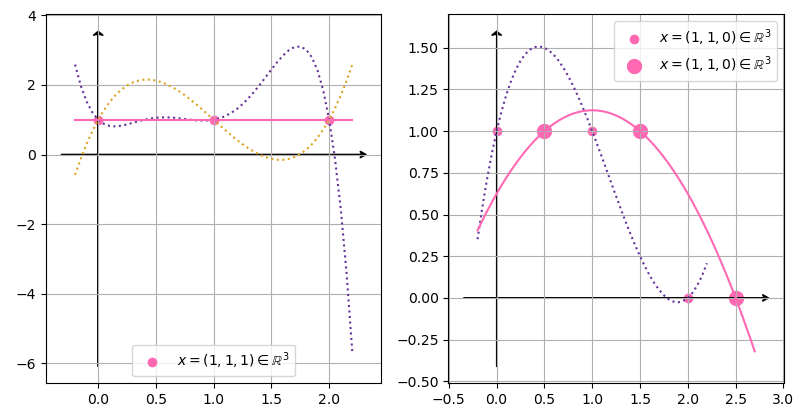
\includegraphics[scale=0.52]{25Nov_1} 
\end{figure}	


\begin{prop}
\label{prop: igualdad de grado (menor a n) si dos polinomios al discretizarse dan x}
Sean $n \in \IN$, $x \in \IR^{n}$.
Si $\cali{P}, \tilde{\cali{P}}$ son mallas uniformes
de $n$ puntos y $\tilde{f}, f \in \IR_{n-1}[x]$
son tales que
\begin{equation}
\label{eq2: 25Nov}
\Omega_{n, \tilde{\cali{P}}}(\tilde{f})= x = 
\Omega_{n, \cali{P}}(f),
\end{equation}
entonces $\partial(\tilde{f})=\partial(f)$.
\end{prop}
\noindent
\textbf{Demostración.}
Digamos que 
\[
\cali{P}=\{t_{j}:=t_{0}+hj: \hspace{0.2cm} 0 \leq j \leq n-1 \},
\hspace{0.2cm}
\cali{\tilde{P}}=\{
\tilde{t_{j}}:=\tilde{t_{0}}+ \tilde{h}j: \hspace{0.2cm} 0 \leq j \leq n-1 \}.
\]
Sea 
\[
\phi(t)= \frac{h}{\tilde{h}}t+ \left( t_{0}-  \frac{h}{\tilde{h}}
\tilde{t_{0}}  \right)
\]
la función de cambio de malla
(de $\tilde{\cali{P}}$ a $\cali{P}$); esta función es 
tal que
\[
\forall \hspace{0.1cm} 0 \leq j \leq n-1, 
\hspace{0.5cm} \phi(\tilde{t_{j}})= 
t_{j};
\]
podemos reescribir entonces la hipótesis \eqref{eq2: 25Nov}
como 
\begin{align*}
(\tilde{f}(\tilde{t_{0}}), \ldots , \tilde{f}(\tilde{t_{n-1}}))
= & x \\
=& (f(t_{0}), \ldots , f(t_{n-1})) \\
=& ((f \circ \phi) (\tilde{t_{0}}), \ldots , 
(f \circ \phi) (\tilde{t_{n-1}})),
\end{align*}
o sea, como $\Omega_{n, \tilde{\cali{P}}}(\tilde{f})=
\Omega_{n, \tilde{\cali{P}}}(f \circ \phi)$; por linealidad
del operador $\Omega_{n, \tilde{\cali{P}}}$
(c.f. observación 
\ref{obs:linealidad de omega restringida a R[x]})
tenemos entonces que
$\Omega_{n, \tilde{\cali{P}}}(\tilde{f}-f \circ \phi)=0$,
o sea, que 
$\tilde{f}-f \circ \phi$ es un polinomio de
grado menor a $n$ con al menos $n$ raíces 
(a saber, los $n$ elementos de $\tilde{\cali{P}}$), luego, 
según la proposición \ref{prop: cita TFA},
$\tilde{f}-f \circ \phi$
es el polinomio cero, por lo tanto, 
\begin{equation*}
\label{eq3: 25Nov}
\tilde{f}=f \circ \phi.
\end{equation*}

Puesto que el componer a $f$ con el polinomio lineal
$\phi$ no altera su grado (i.e. $f$ y $f \circ \phi$
son polinomios del mismo grado), concluimos que
\[
\partial(\tilde{f})= \partial(f \circ \phi)=
\partial(f).
\]
\QEDB
\vspace{0.2cm}

Con todo esto demostrado, podemos definir
el grado de una señal finita como sigue.

\begin{defi}
\label{def: del grado de una senial finita}
Sean $n \in \IN$, $x \in \IR^{n}$.
Si $f \in \IR_{n-1}[x]$
es un polinomio de grado menor a $n$
y $\cali{P}$ es una malla uniforme
de $n$ puntos tales que
$x= \Omega_{n, \cali{P}}(f)$, entonces
el \textbf{grado de $x$} es 
\[
\partial(x):= \partial(f).
\]
\end{defi}


Es fácil determinar el grado de una señal 
de dimensión $n$
en términos de pertencia a los espacios $W_{n,i}$;
mostramos a continuación que
el grado $i$ de un polinomio discreto es el índice
del menor subespacio $W_{n,i}$ en el que está contenido.

\begin{prop}
Sean $n \in \IN$ y $x \in \IR^{n}$ una señal de dimensión $n$.
\begin{itemize}
\item $x$ tiene grado cero si y sólo si $x \in W_{n,0}$.
\item Para toda $1 \leq i \leq n-1$,
$x$ tiene
grado $i$ si y sólo si 
$x \in W_{n,i}$ pero $x \not\in W_{n,i-1}$.
\end{itemize}
\end{prop}
\noindent
\textbf{Demostración.}
La veracidad del primer punto de la demostración
es obvia (pues $W_{n,0}$ consta exactamente de las discretizaciones
puntuales de polinomios constantes, c.f. 
teorema \ref{cor: propiedades importantes de espacios Wi}).
Demostremos pues el segundo punto.

\begin{itemize}
\item [$\Rightarrow$)]

Supongamos que $\partial(x)=i$ con $1 \leq i \leq n-1$;
por definición, esto significa que existen
$\cali{P}$ una malla uniforme de $n$ puntos y $f$ un 
polinomio 
tales que 
\begin{equation}
\label{eq5: 25Nov}
\partial(f)=i \hspace{0.2cm} \text{y} \hspace{0.2cm}
x=\Omega_{n,\cali{P}}(f).
\end{equation}
Según la proposición 
\ref{Obs1},
esto implica la pertenencia de $x$ a $W_{n,i}$.
Además, $x$ no puede ser elemento de $W_{n,i-1}$,
pues esto,
según el tercer punto del corolario
\ref{cor: propiedades importantes de espacios Wi},
implicaría la existencia de una
malla uniforme $\tilde{\cali{P}}$ de $n$
puntos y un polinomio $g$ tales que
\begin{equation}
\label{eq6: 25Nov}
\partial(g)\leq i-1 \hspace{0.2cm} \text{y} \hspace{0.2cm}
x=\Omega_{n,\tilde{\cali{P}}}(g);
\end{equation}
según la proposición
\ref{prop: igualdad de grado (menor a n) si dos polinomios al discretizarse dan x}, \eqref{eq5: 25Nov}
y \eqref{eq6: 25Nov} no pueden ser ambas verdaderas.

\item[$\Leftarrow$)] Sea
$1 \leq i \leq n-1$ tal que $x \in W_{n,i}$
pero $x \not\in W_{n,i-1}$.
Según el corolario
\ref{cor: propiedades importantes de espacios Wi}, existen
$\cali{P}$ malla uniforme de $n$ puntos y
$f$ polinomio de grado a lo más $i$ tales que
$x= \Omega_{n, \cali{P}}(f)$; según este mismo
corolario, el que el grado de $f$ fuese menor a $i$
implicaría que $x$ también fuese elemento
del espacio $W_{n,i-1}$. Como esto no ocurre, concluimos
que $x= \Omega_{n, \cali{P}}(f)$
con $\partial(f)=i$, luego, según la definición
\ref{def: del grado de una senial finita}, 
$x$ tiene grado $i$.
\end{itemize}
\QEDB
\vspace{0.2cm}




\subsection{Construcción de la base de Legendre discreta via ortogonalización de bases de espacios de polinomios discretos}

\noindent Ahora, con el proceso de Gram-Schmidt \ref{Prop:Gram-Schmidt2}
vamos a normalizar
a la base $\{v_{k}: \hspace{0.1cm} 0 \leq k \leq n-1 \}$ de
$W_{n,n-1}$, o sea, de $\IR^{n}$ (c.f. 
cuarto punto del teorema
\ref{cor: propiedades importantes de espacios Wi}). 
Por la naturaleza del proceso, durante este se
obtienen bases ortonormales para cada uno de los espacios 
$W_{n,i}$. \TODO{detalla mejor esto.}

%\begin{figure}[H]
%   \centering
%   \incfig{28JunioInks}
%    \caption{ 
%    \TODO{Cambiar notación espacios W}
%    Como muestra el diagrama, 
%	lo que se hace es proyectar el vector $v_{k}$, con
%	$1 \leq k \leq n-1$, al espacio
%	$W_{n,k-1}$ para así 
%	formar al vector $\bar{\xi}_{k}$ y después
%	normalizarlo.}
%\end{figure}


\begin{defi} 
\label{def: base de Legendre discreta}
A la base ortonormal de $\IR^{n}$
\begin{equation}
\label{eq: base de Legendre discreta}
\cali{L}^{n}=\{ \cali{L}^{n,k}= (\cali{L}_{m}^{n,k})_{m=0}^{n-1} \in \IR^{n}: 
\hspace{0.1cm} 0 \leq k \leq n-1\}
\end{equation}
que resulta de ortonormalizar con G-S a la base
\[
\{v_{k} \in \IR^{n}: \hspace{0.1cm} 0 \leq k \leq n-1 \}
\]
de $\IR^{n}$ la llamaremos la
\textbf{base de Legendre discreta de dimensión $n$}.

Denominaremos a la señal $\cali{L}^{n,k}$ el 
\textbf{polinomio discreto de Legendre de dimensión
$n$ y grado $k$}.
\end{defi}

\begin{cor} \label{cor: BON de legendre para espacios Wk}
Sea $n \in \IN$. Para todo $0 \leq k \leq n-1$, los vectores
\[
\cali{L}^{n, l}, \hspace{0.2cm} 0 \leq l \leq k
\]
conforman una BON del espacio $W_{n,k}$.
\end{cor}

\begin{cor} \label{cor: Ln,k ortogonal a todo pol discreto de grado menor a k}
Sea $n \in \IN$. Si $k$ es un entero con $1 \leq k \leq n-1$,
entonces
\[
\forall \hspace{0.1cm} 0 \leq l \leq k-1:
\hspace{0.2cm}
\cali{L}^{n,k} \in W_{n,l}^{\perp},
\]
o sea, 
$\cali{L}^{n,k}$ es ortogonal a todo polinomio discreto
de grado menor a $k$.
\end{cor}
\noindent
\textbf{Demostración.}
En efecto, según la definición
\ref{def: base de Legendre discreta}, 
$\cali{L}^{n,k}$ es ortogonal a todos los vectores
$\cali{L}^{n, l}$ con $0 \leq l \leq k$,
luego, según el corolario
\ref{cor: BON de legendre para espacios Wk},
ortogonal a toda una base del espacio $W_{n,k}$,
por lo tanto, a todo elemento de este.
\QEDB
\vspace{0.2cm}



\begin{center}
{\Huge{
$\cali{L}^{\textcolor{ameMorado}{n}, 
\textcolor{ameDorado}{k}}=
\left(
\cali{L}^{\textcolor{ameMorado}{n}, 
\textcolor{ameDorado}{k}}_{\textcolor{ameRosa}{m}}
\right)_{m=0}^{m=n-1} \in \IR^{n}
$}}
\end{center}
\begin{itemize}
\item \textcolor{ameMorado}{n} $\in \IN$: dimensión del espacio ambiente
\item $0 \leq  \textcolor{ameDorado}{k} \leq n-1$ entero: parámetro de grado
\item $0 \leq \textcolor{ameRosa}{m} \leq n-1$ entero: parámetro de posición
\end{itemize}
\TODO{Hacer eso una imagen. Tratamos de usar consitentemente la notación
explicada en la figura a lo largo del texto.}